\begin{ejercicio}[
  id=GEO_TRI_001,
  materia=geometria,
  capitulo=triangulos,
  nivel=intermedio,
  procedencia="Examen UNI 2024",
  visibilidad=true,
  libros={geometria_pre, geometria_avanzado},
  youtube_url="https://www.youtube.com/watch?v=ejemplo_geometria_tri",
  mostrar_solucion=true,
  libro_promocion=""
]
En el triángulo $ABC$ mostrado en la figura, se tiene que $AB = 6$ cm, $BC = 8$ cm y $AC = 10$ cm. Si $D$ es el punto medio de $BC$ y $E$ es el punto medio de $AC$, determina la longitud del segmento $DE$.

\begin{center}
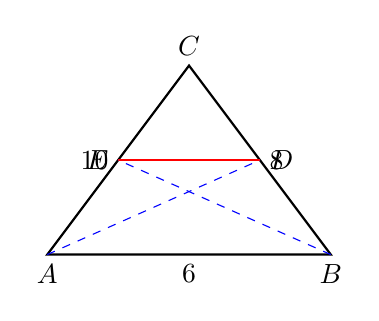
\begin{tikzpicture}[scale=0.6]
\coordinate (A) at (0,0);
\coordinate (B) at (6,0);
\coordinate (C) at (3,4);
\coordinate (D) at (4.5,2);
\coordinate (E) at (1.5,2);

\draw[thick] (A) -- (B) -- (C) -- cycle;
\draw[red, thick] (D) -- (E);
\draw[dashed, blue] (A) -- (D);
\draw[dashed, blue] (B) -- (E);

\node[below] at (A) {$A$};
\node[below] at (B) {$B$};
\node[above] at (C) {$C$};
\node[right] at (D) {$D$};
\node[left] at (E) {$E$};

\node[below] at (3,0) {$6$};
\node[right] at (4.5,2) {$8$};
\node[left] at (1.5,2) {$10$};
\end{tikzpicture}
\end{center}

\begin{solucion}
Para resolver este problema, utilizamos el teorema de la línea media:

1) \textbf{Identificamos los datos:}
   \begin{itemize}
   \item $AB = 6$ cm
   \item $BC = 8$ cm
   \item $AC = 10$ cm
   \item $D$ es punto medio de $BC$
   \item $E$ es punto medio de $AC$
   \end{itemize}

2) \textbf{Aplicamos el teorema de la línea media:}
   La línea que une los puntos medios de dos lados de un triángulo es paralela al tercer lado y mide la mitad de su longitud.

3) \textbf{Calculamos:}
   Como $DE$ es la línea media que une los puntos medios de $BC$ y $AC$, entonces:
   $$DE \parallel AB \text{ y } DE = \frac{AB}{2} = \frac{6}{2} = 3 \text{ cm}$$

4) \textbf{Verificamos con el teorema de Pitágoras:}
   \begin{itemize}
   \item $AB^2 + BC^2 = 6^2 + 8^2 = 36 + 64 = 100 = 10^2 = AC^2$
   \item El triángulo es rectángulo en $B$
   \end{itemize}

\textbf{Respuesta:} La longitud del segmento $DE$ es $3$ cm.

\textbf{Nota:} La figura muestra claramente la relación entre los puntos medios y confirma que $DE$ es paralela a $AB$.
\end{solucion}
\end{ejercicio} 